\documentclass[11pt,a4paper]{article}
\usepackage[utf8]{inputenc}
\usepackage[T1]{fontenc}
\usepackage[english]{babel}
\usepackage[margin=2.1cm]{geometry}
\usepackage{booktabs,array,tabularx}
\usepackage{xcolor}
\usepackage{graphicx}
\usepackage{pgfplots}
\pgfplotsset{compat=1.17}
\PassOptionsToPackage{hyphens}{url}
\usepackage[hidelinks]{hyperref}
\usepackage{enumitem}
\setlist{nosep,leftmargin=1.4em}
\emergencystretch=3em

\definecolor{impl}{HTML}{3B6EA8}
\definecolor{rev}{HTML}{8FB3DA}

\title{Sweatshop on P-Chess: the last three open tickets\\\large Release on \texttt{v*} tags (CI-003) and two test-harness cleanups (CLEAN-007, CLEAN-008); GPT-6.1 Sol lineup}
\author{Foreman, session \texttt{sweatshop/2026-10-25-1843}}
\date{25 October 2026}

\begin{document}
\maketitle

\section*{Summary}

A lane-less run on the main checkout, default lineup \texttt{sol} (stage 2
\texttt{gpt-6.1-sol high}, stage 3 \texttt{gpt-6.1-sol xhigh}). Before launch the proxy (Opus)
triaged CLEAN-007 and CLEAN-008 through \texttt{grill-proxy} (stage 1), with nothing escalated
(\texttt{13503f5} on \texttt{main}). The first launch at 18:43 was stopped by the foreman after
one stage (see \emph{Driver and runtime issues}); the relaunch at 18:50 ended at 19:19 with
``Nothing runnable''.

\begin{itemize}
  \item \textbf{Produced:} CLEAN-007 and CLEAN-008 merged on the session, both
        \texttt{Review: agent}, \texttt{Verdict: Approve}, 0 findings. CI-003 implemented and
        reviewed with 0 findings, but \texttt{blocked}: criterion~5 (a game against Maia from the
        release ZIP on a clean Windows machine) needs Bruno. Session PR
        \href{https://github.com/Laginho/P-Chess/pull/18}{\#18}; gate 254 passed, 0 failed
        (253 on \texttt{main} before the run); PR CI green on Linux and the Windows export.
  \item \textbf{Cost:} \textbf{\$4.18} at API list price over 7 stages:
        \texttt{gpt-6.1-sol xhigh} \$2.29 (review), \texttt{gpt-6.1-sol high} \$1.89 (stage 2).
        Codex quota: 4 points of the weekly window (\texttt{gpt-6.1-sol xhigh} 3,
        \texttt{gpt-6.1-sol high} 1); no thread outside the stages, no window reset.
  \item \textbf{What went wrong:} four local branches left from earlier PRs (pre-rebase copies)
        made the driver re-review CLEAN-002, already \texttt{done}; \$0.11 and one revert.
  \item \textbf{Provisional verdict:} cheap and clean (\$1.40 per ticket on average, 7--15~min
        per ticket end to end). The open item is a human playtest, not a defect.
\end{itemize}

\section*{What was done}

\textbf{CLEAN-007}: nothing changes for players. Two scene-test harnesses,
\path{tests/test_review.gd} and \path{tests/test_clock_input_order.gd}, now clean their isolated
History folder with the shared \texttt{HistoryStorage.clean} instead of a copied loop. No test
added or removed; gate count unchanged.

\textbf{CLEAN-008}: nothing changes for players. A test that awaits a signal that never fires
now fails after 10~s (``timed out after 10 s'') and the run goes on, instead of hanging CI until
its 15-minute kill. \path{tests/run.gd} bounds each awaited test by wall clock;
\path{tests/test_runner.gd} runs its child Godot through a pipe with a 60~s kill. The gate is
about 20~s slower (two child runs wait out the bound).

\textbf{CI-003}: pushing a \texttt{v*} tag builds the Windows app, downloads Lc0 and the nine
Maia nets with their pinned hashes, adds both licences and \path{THIRD_PARTY.md}, and attaches
\path{P-Chess-windows-x86_64.zip} to a GitHub release named after the tag
(\path{.github/workflows/release.yml}). The test tag \texttt{v0.0.1-rc1} produced
\href{https://github.com/Laginho/P-Chess/releases/tag/v0.0.1-rc1}{a public release} (99.7~MB).
The exported app started on this machine with a fresh profile and launched its bundled Lc0; no
game was played (Computer Use refused the window).

\section*{Timeline}

\begin{tabularx}{\linewidth}{@{}lX@{}}
\toprule
18:38 & Proxy (Opus) triages CLEAN-007 and CLEAN-008; \texttt{13503f5} pushed to \texttt{main}. \\
18:43 & Launch, pid 28244; session \texttt{sweatshop/2026-10-25-1843}. Tree lists CLEAN-002/004/005/006 as \texttt{to-review}; CLEAN-002 review starts. Foreman writes \texttt{STOP}. \\
18:44 & CLEAN-002 review: already done via PR \#11, no change. Driver parks it \texttt{blocked} on the session (\texttt{98493d4}), opens PR \#18, stops. \\
18:50 & Proxy (Opus): rename the four stale branches to \texttt{recovery/stale/20261025/*}, revert \texttt{98493d4} (\texttt{ad20d5d}), relaunch after a dry run. Relaunch, pid 28180. \\
18:57 & CLEAN-007 merged, 0 findings. \\
19:05 & CLEAN-008 merged, 0 findings. \\
19:14 & CI-003 to review; release \texttt{v0.0.1-rc1} published by the test tag. \\
19:19 & CI-003 review: 0 findings, \texttt{blocked} on criterion 5 (proxy escalated); ``Nothing runnable''. \\
\bottomrule
\end{tabularx}

\section*{Per stage}

{\small
\begin{tabularx}{\linewidth}{@{}llllrrrrrX@{}}
\toprule
When & Ticket & Stage & Model & Min & In & Cache & Out & Cost & Outcome \\
\midrule
18:44 & CLEAN-002 & review & sol xhigh & 1 & 0.2M & 81\% & 1k & 0.11 & to-review (stale) \\
18:53 & CLEAN-007 & impl & sol high & 3 & 1.2M & 94\% & 6k & 0.43 & to-review \\
18:57 & CLEAN-007 & review & sol xhigh & 4 & 1.6M & 91\% & 12k & 0.69 & merged \\
19:02 & CLEAN-008 & impl & sol high & 5 & 1.5M & 96\% & 8k & 0.48 & to-review \\
19:05 & CLEAN-008 & review & sol xhigh & 3 & 1.1M & 87\% & 9k & 0.57 & merged \\
19:14 & CI-003 & impl & sol high & 10 & 3.2M & 97\% & 18k & 0.98 & to-review \\
19:19 & CI-003 & review & sol xhigh & 5 & 1.9M & 88\% & 14k & 0.91 & blocked \\
\midrule
 & & & & 31 & 10.7M & & 68k & 4.18 & \\
\bottomrule
\end{tabularx}
}

\begin{center}
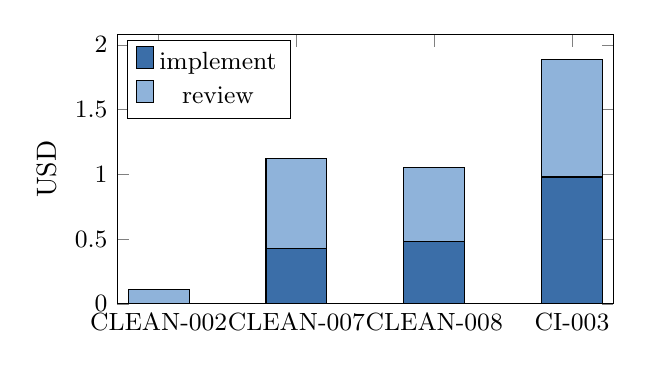
\begin{tikzpicture}
\begin{axis}[ybar stacked, bar width=22pt, width=0.65\linewidth, height=5cm,
  symbolic x coords={CLEAN-002,CLEAN-007,CLEAN-008,CI-003},
  xtick=data, ylabel={USD}, ymin=0, legend style={at={(0.02,0.98)},anchor=north west,font=\small},
  tick label style={font=\small}]
\addplot[fill=impl] coordinates {(CLEAN-002,0) (CLEAN-007,0.43) (CLEAN-008,0.48) (CI-003,0.98)};
\addplot[fill=rev] coordinates {(CLEAN-002,0.11) (CLEAN-007,0.69) (CLEAN-008,0.57) (CI-003,0.91)};
\legend{implement, review}
\end{axis}
\end{tikzpicture}
\end{center}

Wasted: the CLEAN-002 review (\$0.11, 2.6\% of the run), caused by the stale branches.

\section*{Comparison with previous runs}

From \texttt{run-log.md}: the core lane's rework of PR \#10 earlier today cost \$4.10 for three
tickets; this run \$4.18 for three tickets plus the stale review. CI-003 is the most expensive
ticket of the run (\$1.89) because stage 2 waited for a real Actions release and downloaded and
re-verified the ZIP.

\section*{Observations per model}

\begin{itemize}
  \item \textbf{gpt-6.1-sol high, stage 2}: three handoffs at the first attempt, 3--10~min.
        CLEAN-008 committed its red test before the fix. CI-003 pushed the ticket's test tag
        and verified the published asset digest, the 19 pinned engine files and a failing
        package check.
  \item \textbf{gpt-6.1-sol xhigh, review}: three reviews, 0 findings, no code in review (no
        round-0 rows). Two reviews reused the stage-2 gate receipt instead of rerunning the
        gate (allowed for unchanged code). The CLEAN-008 review did not discuss the new test's
        upper bound (child must finish in under 12~s), a possible flake on a slow CI runner;
        Linux CI passed this time.
\end{itemize}

\section*{Driver and runtime issues}

\begin{enumerate}
  \item The main checkout kept four local branches (\texttt{clean-002}, \texttt{clean-004},
        \texttt{clean-005}, \path{CLEAN-006-main-rematch-lifecycle-tests}) that are pre-rebase
        copies of PRs \#11, \#12, \#15 and \#16: same commits by \texttt{git cherry}, different
        hashes. The driver's \texttt{Ticket()} reads \texttt{Stage:} from any unmerged branch
        matching the id unless the session says \texttt{blocked}, so the four \texttt{done}
        tickets read as \texttt{to-review}. Earlier runs used lane clones, which never had these
        branches. Not patched; follow-up for the sweatshop skill.
  \item \texttt{.scratch/run-log/} was missing from the main checkout's
        \texttt{.git/info/exclude}; the foreman added it before launch.
\end{enumerate}

\section*{Recommendations}

\begin{enumerate}
  \item Sweatshop driver: treat a ticket branch as merged when the session says \texttt{done}
        and \texttt{git cherry <base> <branch>} shows no unique patch.
  \item Run foreman lanes in clones, or prune merged-by-rebase local branches before a
        lane-less run on the main checkout.
  \item Keep the \texttt{sol} lineup for small tickets: scoreboard row \texttt{gpt-6.1-sol high}
        $\rightarrow$ \texttt{gpt-6.1-sol xhigh}, 18 reviews, 22\% reopened, S2 rate 22\%.
\end{enumerate}

\section*{Human debt and proxy decisions}

No \texttt{Débito humano:} lines. Proxy decisions of this run:

\begin{itemize}
  \item \textbf{CLEAN-007} (Opus, stage 1): ``narrow scope, test\_review + test\_clock\_input\_order
        switch to \texttt{HistoryStorage.clean}; helper, test\_badges, test\_book unchanged'';
        ``no red test'' (CLEAN-003 precedent); ``do it, low priority (not wontfix)'';
        ``Status ready-for-agent, Stage to-implement, Blocked by none''.
  \item \textbf{CLEAN-008} (Opus, stage 1): ``10 s wall-clock bound per awaited
        \texttt{test\_*}, a constant in run.gd, no CLI flag''; ``timeout = FAIL, counted, run
        continues; the suspended coroutine is abandoned''; ``bound \texttt{\_run} itself in
        test\_runner.gd \ldots\ waiting synchronously with a kill deadline of about 60 s'';
        ``criteria and Primary files confirmed as drafted''.
  \item \textbf{CLEAN-002/004/005/006} (Opus, run anomaly): rename the stale branches, revert
        \texttt{98493d4}, relaunch on the same session.
  \item \textbf{CI-003}: \texttt{Proxy escalated (gpt-6-astra high, fallback)} by the review
        stage: criterion 5 cannot be waived without a clean-Windows game.
\end{itemize}

\section*{Reopen attribution}

No reopened review and no fix made in review in this run, so no new rows in
\path{reopen-attribution.md}. No session-review, release-audit or post-release finding was
reported since the last pass.

\section*{Scoreboard}

\texttt{scoreboard.ps1} over P-Chess, ClassyCall, EasyMath, PhysiSyst, SIGAA-ME and
SynchroNice main checkouts (no lane clone). Rows for this lineup: \texttt{gpt-6.1-sol high}
$\rightarrow$ \texttt{gpt-6.1-sol xhigh} 18 reviews, 4 reopened (22\%), S2 rate 22\%;
\texttt{gpt-6.1-sol xhigh} $\rightarrow$ \texttt{gpt-6.1-sol xhigh} 6 reviews, 1 reopened (an
anecdote). The previous report printed 105 reviews for the first pair from a lane clone, whose
copied-back log counts rows twice; the two figures do not compare. Interventions:
proxy-decision (opus) 30, routine approvals 18, human rescues 24.

\section*{Pending for the human}

\begin{enumerate}
  \item CI-003 criterion 5: unzip the
        \href{https://github.com/Laginho/P-Chess/releases/tag/v0.0.1-rc1}{\texttt{v0.0.1-rc1}}
        ZIP on a clean Windows machine and play one game against Maia; report the Windows
        version and the result. Then CI-003 returns to \texttt{to-review}.
  \item Release \texttt{v0.0.1-rc1} is public, not marked pre-release and shown as ``Latest'':
        keep, mark pre-release, or delete.
  \item Review and merge session PR \#18 (CLEAN-007, CLEAN-008).
  \item The CI-002 note on CI-003 (the missing-engine message points at
        \path{scripts/fetch-engine.ps1}, which an export does not ship) was not acted on.
  \item The four \texttt{recovery/stale/20261025/*} branches can be deleted at your call.
\end{enumerate}

\end{document}
